\documentclass{article}
\usepackage[UTF8]{ctex}
\usepackage{graphicx}
\usepackage[a4paper, margin=1in]{geometry}
\usepackage{amsmath}
\usepackage{algorithm}
\usepackage{algorithmic}
\usepackage{pdfpages}
\begin{document}

\title{\Huge 数据挖掘——论文阅读}
\date{\today}

\maketitle

\begin{center}
    \begin{tabular}{ll}
        姓名:   & 杨筠松                                    \\
        学号:   & U202115980                             \\
        学院:   & 电子信息与通信学院                              \\
        邮箱:   & shinehale730@gmail.com                 \\
        论文题目: & Self-supervised Discriminative Feature
        \\ & Learning for Deep Multi-view Clustering \\
        论文出处: & IEEE Transactions on Knowledge         \\
              & and Data Engineering                   \\
              & ( Volume: 35, Issue: 7, 01 July 2023)
    \end{tabular}
\end{center}

\newpage

\tableofcontents

\newpage

\section{原文翻译}

\subsection{摘要}

多视图聚类是一个重要的研究课题, 因为它能够利用多个视图中的互补信息。
然而, 很少有方法考虑到某些视图由于聚类结构不清晰而导致的负面影响, 结果是多视图聚类性能较差。

为了解决这一缺点, 我们提出了用于深度多视图聚类的自监督判别特征学习方法(SDMVC)。
具体来说, 深度自编码器被应用于独立地学习每个视图的嵌入特征。
为了利用多视图的互补信息, 我们将所有视图的嵌入特征拼接起来形成全局特征, 从而克服某些视图聚类结构不清晰所带来的负面影响。
以自监督的方式,我们获取伪标签来构建一个统一的目标分布,以执行多视图判别特征学习。

在此过程中, 可以挖掘全局判别信息来监督所有视图学习更具判别性的特征, 这些特征反过来又用于更新目标分布。

此外, 这个统一的目标分布可以使SDMVC学习一致的聚类分配, 实现多个视图的聚类一致性, 同时保留其特征的多样性。
在各种类型的多视图数据集上的实验表明, SDMVC达到了最先进的性能。

\subsection{导引}

作为一项基础任务, 聚类分析已被应用于广泛领域, 如机器学习、计算机视觉、数据挖掘和模式识别等。然而, 传统的聚类方法通常不适用于现实世界数据来自多个视图或模态的场景, 例如:
\begin{enumerate}
    \item 一个对象的多个映射,
    \item 视觉特征 + 文本特征,
    \item 尺度不变特征变换(SIFT)+ 局部二值模式(LBP)。
\end{enumerate}
因此, 多视图聚类(MVC)成为一个热门研究课题, 可以访问多视图数据中隐藏的互补信息和综合特征。MVC 大致可以分为四类:
\begin{enumerate}
    \item 许多 MVC 方法基于子空间聚类, 其中探索了多个视图的共享表示和相似性度量矩阵。
    \item 一些 MVC 方法通过非负矩阵分解将每个视图分解成一个低秩矩阵进行聚类。
    \item 在第三类 MVC 中, 图结构信息被整合来挖掘多个视图之间的聚类。
    \item 近年来, 深度学习技术也被应用于 MVC, 深度 MVC 旨在通过深度模型的特征表示能力获得更好的性能。
\end{enumerate}
尽管现有的 MVC 方法在过去十年中取得了显著进展, 但其性能在以下问题上仍然有限。首先, 一些 MVC 方法依赖于过多的超参数, 但在实际的聚类应用中, 没有标签信息可以用来调整它们。此外, 许多 MVC 方法复杂度高, 因此难以解决大规模数据聚类任务。此外, 先前的工作通常在嵌入特征空间中直接实现多个视图的一致性, 这降低了特征保持多个视图之间多样性的能力。其结果是, 如果某些视图的聚类结构非常模糊, 清晰聚类结构的视图效果会受到限制, 从而导致聚类性能较差。

为了克服上述问题, 我们提出了用于深度多视图聚类的自监督判别特征学习(SDMVC)。
我们的动机来自图1所示的观察:
\begin{enumerate}
    \item 由于视图的多样性, 多个视图的判别能力是不同的(例如, 从颜色视角来看, 红色摩托车和红色自行车几乎无法区分, 但从语义视角来看, 它们是显然可区分的)。因此, 不同视图特征的判别程度不同, 更高的判别特征更有利于聚类(即, 更高判别特征具有更清晰的聚类结构)。
    \item 当特征被拼接时, 具有高判别力的聚类结构在划分全局特征空间中起主要作用, 这可以产生高置信度的伪标签并克服聚类结构不清晰的负面影响。
    \item 伪标签可用于引导所有视图学习更具判别力的特征, 从而进一步产生更清晰的聚类结构和更准确的伪标签。
\end{enumerate}

\begin{figure}[h]
    \centering
    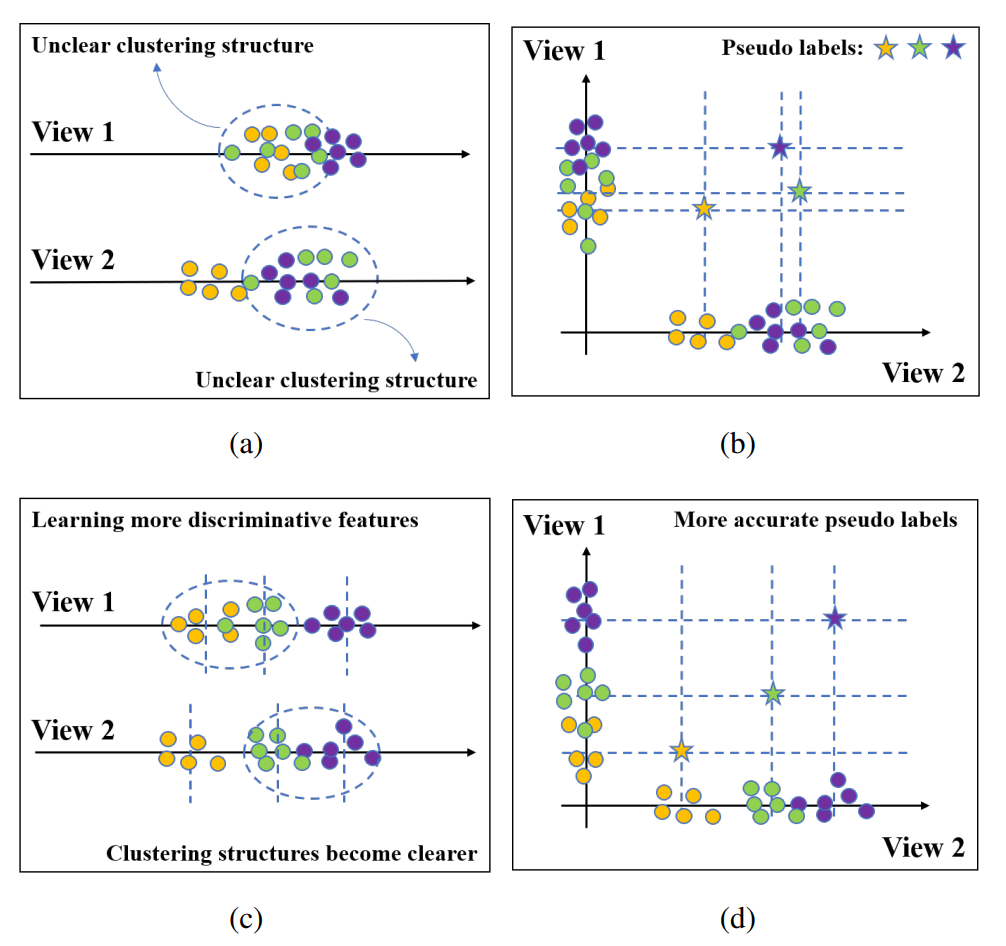
\includegraphics[width=0.75\linewidth]{./imgs/img1.png}
    \caption{视图的多样性示例}
\end{figure}


特别地, 所提出的自监督多视图判别特征学习框架如图2所示。对于每个视图, 使用相应的自编码器通过优化重构损失 \(L_v^r\) 来学习低维嵌入特征 \(z_v\)。不同视图的嵌入特征的判别能力不同。为了利用全局判别信息, 我们将所有嵌入特征连接起来依次构建全局特征、伪标签和统一的目标分布。在此过程中, 可以挖掘特征的互补性并克服聚类结构不清晰的视图带来的负面影响。然后, 通过优化统一目标分布 \(P\) 与每个视图的聚类分配 \(Q_v\) 之间的 KL 散度 \(L_v^c\) 来进行特征学习。通过这种方式, 可以利用全局判别信息引导所有视图学习更多的判别特征, 进而帮助获得互补信息和更准确的目标分布。我们进一步证明了 SDMVC 可以学习一致的聚类分配, 即通过优化具有统一目标分布的多视图聚类损失, 实现所有视图的聚类一致性。此外, 由于提出的每个视图的独立训练, 该框架可以保持所有视图特征的多样性。

总之, 本文的贡献包括:
\begin{itemize}
    \item 我们提出了一种具有新颖自监督多视图判别特征学习框架的深度多视图聚类方法, 该框架可以利用所有视图嵌入特征中包含的全局判别信息来执行多视图聚类。
    \item 从聚类分配而不是特征的角度来看, 该框架实现了多个视图的聚类一致性, 同时保留了其特征的多样性。此外, 它可以克服某些视图聚类结构不清晰对多视图聚类造成的负面影响。
    \item 所提出的方法不依赖于某些超参数, 其复杂度与数据规模成线性关系。不同类型数据集上的实验表明其达到了最先进的聚类性能。
\end{itemize}

\begin{figure}[h]
    \centering
    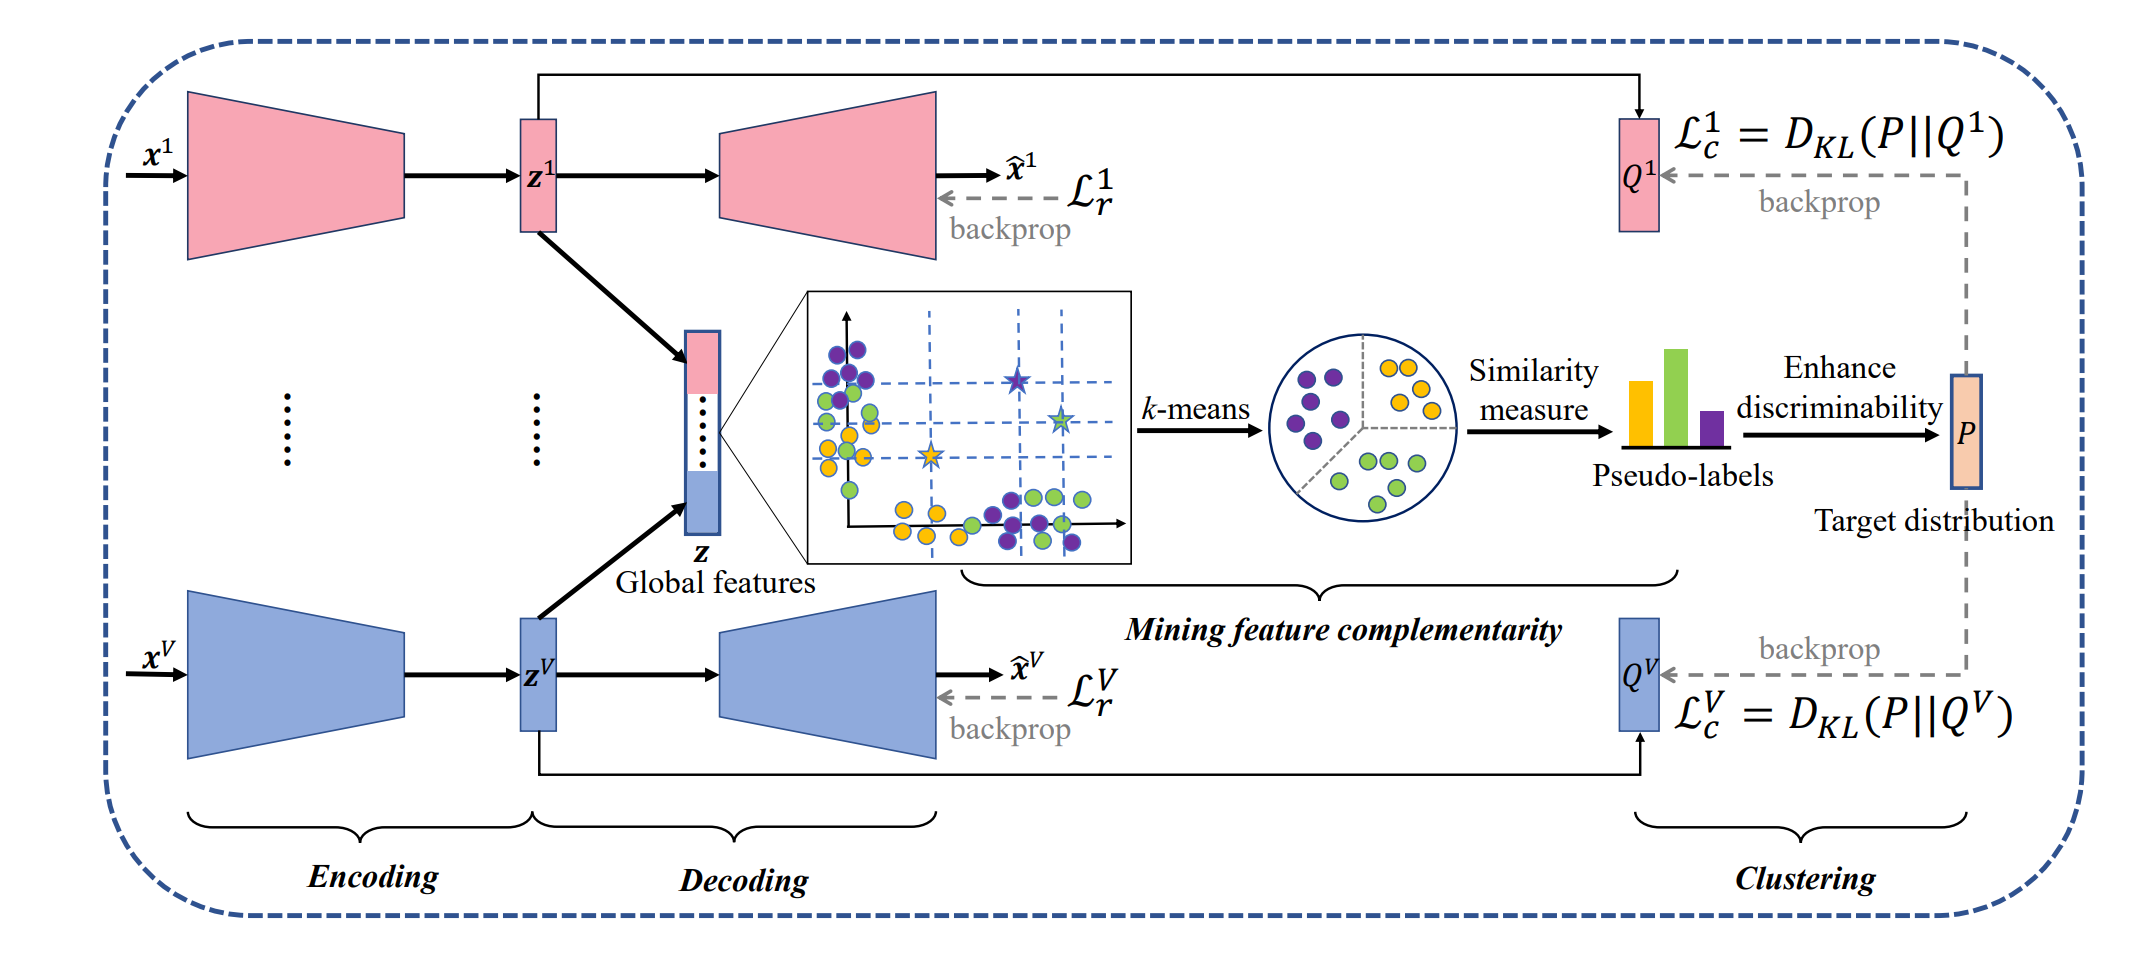
\includegraphics[width=\linewidth]{./imgs/img2.png}
    \caption{SDMVC的框架。每个视图包含一个自编码器和一个聚类层。 \(z_v\) 是嵌入特征,  \(Q_v\) 是聚类分配分布。统一的目标分布 \(P\) 被迭代更新以进行多视图判别特征学习。}
\end{figure}


\subsection{相关工作}

\subsubsection*{深度嵌入聚类}

深度自编码器是流行的深度模型之一,  具有良好的嵌入特征表示能力,  并且其计算复杂度与数据规模成线性关系。
近年来,  基于深度自编码器的聚类被广泛研究。
其中最受欢迎的工作之一是深度嵌入聚类(DEC), 它联合学习自编码器的聚类分配和嵌入特征。
改进的深度嵌入聚类(IDEC)引入了聚类和重构之间的权衡, 以防止嵌入空间的崩溃。
文献[20]中提出的模型是DEC的另一种变体, 它在卷积自编码器上堆叠了多项逻辑回归。
更多基于DEC的研究可以在[21]、[22]、[23]中找到。
尽管许多基于深度神经网络的工作取得了令人印象深刻的表现[18]、[20]、[24]、[25], 这些方法无法处理多视图聚类任务。
在本文中, 我们提出了一种新颖的深度多视图聚类框架, 在该框架中, 判别嵌入特征以自监督方式进行学习

\subsubsection*{多视图聚类}
基于子空间的多视图聚类被广泛讨论, 这种方法假设多个视图的数据来自同一个潜在空间。
在文献[26]中, 作者探讨了使用自表示层来分层重构特定视图的子空间, 并使用编码层使跨视图子空间更加一致。
最近, 在文献[13]和[27]中, 多视图数据被转化为联合表示进行多视图聚类。
另一个研究[28]中, 作者学习了多视图嵌入, 并在学习到的潜在空间中联合挖掘共同结构和聚类分配。
一些多视图聚类方法使用了非负矩阵分解技术, 例如, Liu等人[5]通过该技术探索了多个视图之间的共同潜在因素。
一个深度结构[29]被构建来寻求具有更多一致信息的共同特征。一些方法[8]、[9]、[30]、[31]、[32]利用基于图的模型进行多视图聚类。
例如, 文献[33]提出了一个多图拉普拉斯正则化低秩表示用于多视图谱聚类。
Peng等人[10]通过连接图在投影空间中挖掘几何和聚类对齐一致性。
在文献[34]中, 图自编码器也被引入以学习多视图表示。

一些工作基于其他学习方法。例如, Zhang等人[35]将离散表示学习和二元聚类结合到一个统一框架中。
在文献[36]中, 采用自步学习来防止陷入局部最优。
此外, 深度学习也是一个引人注目的趋势。
例如, Zhu等人[12]训练深度自编码器以获得自表示, 并利用多样性和普遍性正则化来抽象视图间的高阶关系。
基于对抗学习的深度多视图聚类(MVC)在文献[11]、[37]中提出, 旨在学习多视图数据的内在嵌入结构。
自监督学习是当前社区的热门话题。文献[38]提出的框架将自监督范式与多视图聚类相结合。
然而, 它属于子空间聚类, 并依赖于特征值分解, 导致数据规模的三次复杂度。

对于多视图聚类, 获得同一实例的多个视图的一致预测非常重要。
Wang等人[39]最大化了加权视图特定分区与共识分区之间的一致性。
文献[14]引入了参考视图, 以明确训练所有视图以实现一致的预测。
最新的研究[40]在对齐多视图表示分布时引入了两个深度MVC模型。
与以前的方法不同, 我们的方法通过建立统一的目标分布来实现一致的多视图聚类预测。
此外, 自监督多视图判别特征学习框架在我们的工作中首次提出。

\subsection{递交方案}

\subsubsection*{问题描述}

给定一个多视图数据集
\(
\{
x_i^1 \in R^{D_1},
x_i^2 \in R^{D_2},
\ldots,
x_i^V \in R^{D_V}
\}_{i=1}^{N}
\)
其中 V 是视图的总数, N 是样本的数量, D1, D2, \ldots, DV 分别是各个视图的维度。多视图聚类的目标是将样本划分为 K 个簇。

\subsubsection*{A. 自监督多视图判别特征学习}



通常, 一个样本的多个视图在维度或输入形式上是不同的。为了获得便于聚类的特征, 我们使用深度自编码器对每个视图进行特征表示学习。具体来说, 令 $f^v_{\theta_v}$ 和 $g^v_{\phi_v}$ 分别表示第 $v$ 个视图的编码器和解码器。参数 $\theta_v$ 和 $\phi_v$ 实现了第 $v$ 个自编码器的非线性映射, 其编码器部分通过以下公式学习低维特征:

\begin{equation}
    \mathbf{z}^v_i = f^v_{\theta_v}(\mathbf{x}^v_i),
\end{equation}

其中 $\mathbf{z}^v_i \in R^{d_v}$ 是 $\mathbf{x}^v_i$ 在 $d_v$ 维特征空间中的嵌入点。自编码器的解码器部分通过解码 $\mathbf{z}^v_i$ 重构样本 $\hat{\mathbf{x}}^v_i \in R^{D_v}$:

\begin{equation}
    \hat{\mathbf{x}}^v_i = g^v_{\phi_v}(\mathbf{z}^v_i) = g^v_{\phi_v}(f^v_{\theta_v}(\mathbf{x}^v_i)).
\end{equation}

对于每个视图, 优化输入和输出之间的重构损失, 以便将各种形式的输入转换为低维嵌入特征:

\begin{equation}
    L^v_r = \sum_{i=1}^{N} \left\| \mathbf{x}^v_i - g^v_{\phi_v}(f^v_{\theta_v}(\mathbf{x}^v_i)) \right\|^2_2.
\end{equation}

在每个视图的嵌入特征上, 我们构建了一个具有可学习参数 $\{ \boldsymbol{\mu}^v_j \in R^{d_v} \}^K_{j=1}$ 的聚类层 $c^v_{\mu_v}$。$\boldsymbol{\mu}^v_j$ 表示第 $v$ 个视图的第 $j$ 个簇质心。此外, DEC [18] 和 IDEC [19] 是流行的单视图深度聚类方法, 它们使用学生的 t-分布 [41] 生成软聚类分配。类似的方法应用于计算我们的聚类层的输出, 可以描述为:

\begin{equation}
    q^v_{ij} = c^v_{\mu_v}(\mathbf{z}^v_i) = \frac{(1 + \left\| \mathbf{z}^v_i - \boldsymbol{\mu}^v_j \right\|^2)^{-1}}{\sum_j (1 + \left\| \mathbf{z}^v_i - \boldsymbol{\mu}^v_j \right\|^2)^{-1}},
\end{equation}

其中 $q^v_{ij}$ 是第 $i$ 个样本属于第 $j$ 个簇在第 $v$ 个视图中的概率(软聚类分配)。如图 2 所示, 我们的框架有 $V$ 个聚类层和 $V$ 个自编码器。所有视图的嵌入特征都是独立学习的, 这对于学习每个视图的特殊特性是必不可少的, 这些特性可以为多视图聚类提供补充信息。

实际上, 通过公式 (4) 计算的软分配衡量了嵌入特征和簇质心之间的相似性, 因此聚类性能取决于嵌入特征的判别度。由于清晰或不清晰的聚类结构, 不同视图的判别性(判别度)不同。由于嵌入特征 $\mathbf{z}^v_i$ 仅包含第 $v$ 个视图的判别信息, 我们从全局视角出发, 然后定义一个统一的目标分布来进行多视图判别特征学习。具体来说, 为了利用所有视图的判别信息, 我们将所有嵌入特征(缩放到相同范围)连接起来生成全局特征:

\begin{equation}
    \mathbf{z}_i = [\mathbf{z}^1_i; \mathbf{z}^2_i; \ldots; \mathbf{z}^V_i] \in R^{\sum_{v=1}^V d_v}.
\end{equation}

之后, 在全局特征上应用 k-means [42] 计算簇质心:

\begin{equation}
    \min_{\mathbf{c}_1, \mathbf{c}_2, \ldots, \mathbf{c}_K} \sum_{i=1}^{N} \sum_{j=1}^{K} \left\| \mathbf{z}_i - \mathbf{c}_j \right\|^2,
\end{equation}

其中 $\mathbf{c}_j$ 是第 $j$ 个簇质心。然后, 我们应用学生的 t-分布作为核来衡量全局特征 $\mathbf{z}_i$ 和簇质心 $\mathbf{c}_j$ 之间的相似性。相似性用于生成伪软分配(伪标签)$s_{ij}$ 以进行自监督学习, 计算公式为:

\begin{equation}
    s_{ij} = \frac{(1 + \left\| \mathbf{z}_i - \mathbf{c}_j \right\|^2)^{-1}}{\sum_j (1 + \left\| \mathbf{z}_i - \mathbf{c}_j \right\|^2)^{-1}}.
\end{equation}

在应用 k-means 时, 一些高判别性视图的特征在划分全局特征空间时起主要作用, 这保证了伪软分配的准确性, 并克服了低判别性视图中不清晰聚类结构的负面影响。通常, 伪软分配中的高概率成分表示高置信度。为了提高伪软分配的判别性, 我们通过以下公式将其增强为统一目标分布(记作 $P$):

\begin{equation}
    p_{ij} = \frac{(s_{ij})^2/\sum_i s_{ij}}{\sum_j ((s_{ij})^2/\sum_i s_{ij})}.
\end{equation}

为了使所有自编码器学习更高判别性的嵌入特征, $P$ 被用于所有视图的聚类导向损失函数中。具体来说, 对于第 $v$ 个视图, 聚类损失 $L^v_c$ 是统一目标分布 $P$ 和其自身聚类分配分布 $Q^v$ 之间的 Kullback-Leibler 散度(DKL):

\begin{equation}
    L^v_c = DKL(P || Q^v) = \sum_{i=1}^{N} \sum_{j=1}^{K} p_{ij} \log \frac{p_{ij}}{q^v_{ij}}.
\end{equation}

因此, 每个视图的总损失包括两个部分:

\begin{equation}
    L^v = L^v_r + \gamma L^v_c.
\end{equation}

其中 $\gamma$ 是权衡系数。重构损失 $L^v_r$(公式 (3))可以看作是嵌入特征的正则化, 确保低维特征能够保持样本的表示能力。优化聚类损失 $L^v_c$ 使得第 $v$ 个视图的自编码器学习更多判别特征。

因此, 在优化 $\{L^1, L^2, \ldots, L^V\}$ 后, 可以挖掘多视图中包含的更多判别信息。我们进一步利用学习到的特征, 通过公式 (5)–(8) 生成更准确的目标分布。因此, 通过执行所提出的特征学习, 全局判别信息可以用于迭代引导所有视图学习更多判别特征, 尤其是对于那些判别特征较低的视图。最终, 所有视图的嵌入特征的判别性得到提高, 从而获得更清晰的聚类结构。


\subsubsection*{B. 一致的多视图聚类}

在第 $v$ 个视图中, 第 $i$ 个样本的聚类预测通过以下公式计算:

\begin{equation}
    y^v_i = \arg \max_j (q^v_{ij}).
\end{equation}

由于聚类中没有标签信息, 我们甚至不知道哪个视图的聚类预测更准确。但是, 以下定理保证了多视图聚类的一致性, 即多个视图对同一样本具有一致的聚类预测。

定理 1. 通过一个统一的 $P$ 最小化多个 KL 散度, 使得多个视图的 $Q^v$ 趋向一致。

证明. 我们提出的 SDMVC 的多视图聚类损失优化为:

\begin{equation}
    \min_{Q^v} L^v_c = DKL(P || Q^v), \quad v \in \{1, 2, \ldots, V\}.
\end{equation}

对于任意两个视图, $a$ 和 $b \in \{1, 2, \ldots, V\}$, 令 $\xi_a$ 和 $\xi_b$ 表示 $L^a_c$ 和 $L^b_c$ 的优化误差。给定 KL 散度的非负性, 我们得到以下两个不等式:

\begin{equation}
    0 \leq DKL(P || Q^a) = \sum_{i=1}^{N} \sum_{j=1}^{K} p_{ij} \log \frac{p_{ij}}{q^a_{ij}} \leq \xi_a,
\end{equation}

\begin{equation}
    0 \leq DKL(P || Q^b) = \sum_{i=1}^{N} \sum_{j=1}^{K} p_{ij} \log \frac{p_{ij}}{q^b_{ij}} \leq \xi_b.
\end{equation}

公式 (14)+(−公式 (13)), 以下不等式成立:

\begin{equation}
    -\xi_a \leq \sum_{i=1}^{N} \sum_{j=1}^{K} p_{ij} \log \frac{q^a_{ij}}{q^b_{ij}} \leq \xi_b.
\end{equation}

当 $P$ 固定时, 最小化 $\xi_a \to 0$ 和 $\xi_b \to 0$ 导致

\begin{equation}
    \sum_{i=1}^{N} \sum_{j=1}^{K} p_{ij} \log \frac{p_{ij}}{q^a_{ij}} \to 0, \quad 即 \ Q^a \to P,
\end{equation}

\begin{equation}
    \sum_{i=1}^{N} \sum_{j=1}^{K} p_{ij} \log \frac{p_{ij}}{q^b_{ij}} \to 0, \quad 即 \ Q^b \to P,
\end{equation}

并且

\begin{equation}
    \sum_{i=1}^{N} \sum_{j=1}^{K} p_{ij} \log \frac{q^a_{ij}}{q^b_{ij}} \to 0, \quad 即 \ Q^b \to Q^a.
\end{equation}

因此, $Q^a$ 和 $Q^b$ 趋向一致。这个结论可以很容易地推广到多个视图的情况。

定理 1 表明我们的方法可以在多个视图中获得一致的软聚类分配。在此基础上, 平均多个软聚类分配可以避免少数错误预测的干扰, 并实现更高置信度的明确聚类预测。因此, 最终的聚类预测通过以下公式计算:

\begin{equation}
    y_i = \arg \max_j \left( \frac{1}{V} \sum_{v=1}^{V} q^v_{ij} \right).
\end{equation}

考虑到不同视图的多样性, 期望所有视图对所有样本具有一致预测是不合理的。我们定义当 $y^1_i = y^2_i = \cdots = y^V_i$ 时, 第 $i$ 个样本是对齐的。因此, 我们计算所有样本中对齐样本的比例, 称为“对齐率”, 以确定模型的停止条件。由于这也是一个无监督过程, 当达到较高的对齐率时, 我们可以停止训练, 以确保多视图聚类的一致性。

所提出的流程如图 2 所示。总之, 通过设置统一的目标分布, 实现了多视图聚类的一致性。优化 $L^v$ 只影响第 $v$ 个视图的自编码器和聚类层, 因此每个视图的嵌入特征和聚类质心的优化是独立于其他视图的。因此, 所提出的框架可以在保持特征多样性的同时实现多个视图的聚类一致性。


\subsubsection*{C. 优化}


一开始, 自编码器的参数随机初始化。为了获得有效的目标分布, 自编码器通过公式 (3) 进行预训练。之后, 应用 k-means 初始化可学习的聚类质心 $\boldsymbol{\mu}^v_j$。对于第 $v$ 个视图, 要训练的参数是编码器的 $\theta_v$, 解码器的 $\phi_v$ 和聚类层的 $\boldsymbol{\mu}^v_j$。

在判别特征学习过程中, 目标分布 $P$ 是固定的。聚类损失 $L^v_c$ 相对于聚类质心 $\boldsymbol{\mu}^v_j$ 和嵌入特征 $\mathbf{z}^v_i$ 的梯度分别为:

\begin{equation}
    \frac{\partial L^v_c}{\partial \boldsymbol{\mu}^v_j} = 2 \sum_{i=1}^{N} (1 + \left\| \mathbf{z}^v_i - \boldsymbol{\mu}^v_j \right\|^2)^{-1}(q^v_{ij} - p_{ij})(\mathbf{z}^v_i - \boldsymbol{\mu}^v_j)
\end{equation}

和

\begin{equation}
    \frac{\partial L^v_c}{\partial \mathbf{z}^v_i} = 2 \sum_{j=1}^{K} (1 + \left\| \mathbf{z}^v_i - \boldsymbol{\mu}^v_j \right\|^2)^{-1}(p_{ij} - q^v_{ij})(\mathbf{z}^v_i - \boldsymbol{\mu}^v_j).
\end{equation}

我们使用小批量梯度下降和反向传播算法来微调模型。令 $n$ 和 $\lambda$ 分别表示批量大小和学习率。该方法总结如下算法 1。在固定的迭代次数后, 目标分布将被更新, 以便自编码器可以学习更多判别特征。具体实验设置请参见第四节 C 部分。

复杂度分析。$K$、$V$ 和 $N$ 分别是簇的数量、视图的数量和样本的数量。令 $M$ 表示自编码器隐藏层中神经元的最大数量, $Z$ 表示嵌入特征的最大维度。通常 $V, K, Z \ll M$ 成立。k-means 和计算目标分布的复杂度都是 $O(N Z K)$。计算对齐率的复杂度是 $O(N K)$。$V$ 个自编码器的复杂度是 $O(V N M^2)$。总之, 我们算法的复杂度与数据规模 $N$ 成线性关系。

\begin{algorithm}
    \caption{深度多视图聚类的自监督判别特征学习 (SDMVC)}
    \label{alg:SDMVC}
    \begin{algorithmic}[1]
        \REQUIRE 多视图数据集; 簇的数量 $K$; 权衡系数 $\gamma$; 停止阈值 $\delta$.
        \ENSURE 聚类分配 $\mathbf{y}$.
        \STATE 通过公式 (3) 预训练每个视图的深度自编码器.
        \STATE 通过 k-means 初始化每个视图的聚类质心.
        \WHILE {未达到停止条件}
        \STATE 通过公式 (5) 和 (6) 计算全局特征上的质心.
        \STATE 通过公式 (7) 和 (8) 更新目标分布 $P$.
        \STATE 计算 $\{\mathbf{y}^1, \mathbf{y}^2, \ldots, \mathbf{y}^V\}$ 的对齐率.
        \IF {对齐率 > $\delta$}
        \STATE 停止训练.
        \ENDIF
        \FOR {固定目标分布 $P$}
        \STATE 微调所有自编码器的参数:
        \STATE $\boldsymbol{\mu}^v_j = \boldsymbol{\mu}^v_j - \frac{\lambda}{n} \sum_{i=1}^{n} \frac{\partial L^v_c}{\partial \boldsymbol{\mu}^v_j}$,
        \STATE $\phi_v = \phi_v - \frac{\lambda}{n} \sum_{i=1}^{n} \frac{\partial L^v_r}{\partial \phi_v}$,
        \STATE $\theta_v = \theta_v - \frac{\lambda}{n} \sum_{i=1}^{n} \left( \frac{\partial L^v_r}{\partial \theta_v} + \gamma \frac{\partial L^v_c}{\partial \theta_v} \right)$.
        \ENDFOR
        \ENDWHILE
        \STATE 输出通过公式 (19) 计算的 $\mathbf{y}$.
    \end{algorithmic}
\end{algorithm}



\subsection{实验设置}

\subsubsection*{A. 数据集}
MNIST-USPS. MNIST[43]和 USPS 都是手写数字图像数据集。
在多视图聚类中, 它们总是被视为数字的两种不同视图。

我们实验中使用了与[10]相同的数据集, 每个视图包含10个类别, 每个类别提供500个样本。
Fashion-MV. Fashion [44] 包含10种时尚产品(如T恤、连衣裙和外套等)。
我们使用30,000个样本构建Fashion-MV。它有三个视图, 每个视图包含10,000张灰度图像。
每三个从同一类别中抽取的图像构成一个实例的三个视图。BDGP. BDGP [45] 包含关于果蝇胚胎的2,500张图像, 分为5个类别。
每张图像的1,750维视觉特征和79维文本特征用于多视图聚类。
Caltech101-20. 使用了2,386张图像(从一个RGB图像数据集[46]中抽取)构建多视图数据集[35]。
它包含20个类别和六种不同的视图, 即48维Gabor、40维小波矩(WM)、254维CENTRIST、1,984维HOG、512维GIST和928维LBP。
所有数据集的输入特征都被缩放到[0, 1]。

\subsubsection*{B. 比较方法}
我们将SDMVC与以下流行的最先进方法进行比较。

浅层模型包括k-means、SC、BMVC、MVC-LFA、COMIC、GMC和SAMVC。

深层模型包括DEC、IDEC、PVC、EAMC、SiMVC、DEMVC和我们的SDMVC。

单视图方法:k-means [42]、SC(谱聚类[47])、DEC(深度嵌入聚类[18])、IDEC(改进的深度嵌入聚类[19])。对于这些单视图方法, 输入是所有视图的拼接。

多视图方法: BMVC(二进制多视图聚类[35])、MVC-LFA(通过后融合对齐最大化的多视图聚类[39])、COMIC(跨视图匹配聚类[10])、
GMC(基于图的多视图聚类[9])、SAMVC(自步和自动加权的多视图聚类[36])、PVC(部分视图对齐聚类[48])、EAMC(用于多模态聚类的端到端对抗注意力网络[37])、SiMVC和CoMVC(重新考虑表示对齐的多视图聚类[40])、DEMVC(协作训练的深度嵌入多视图聚类[14])。

\begin{figure}[h]
    \centering
    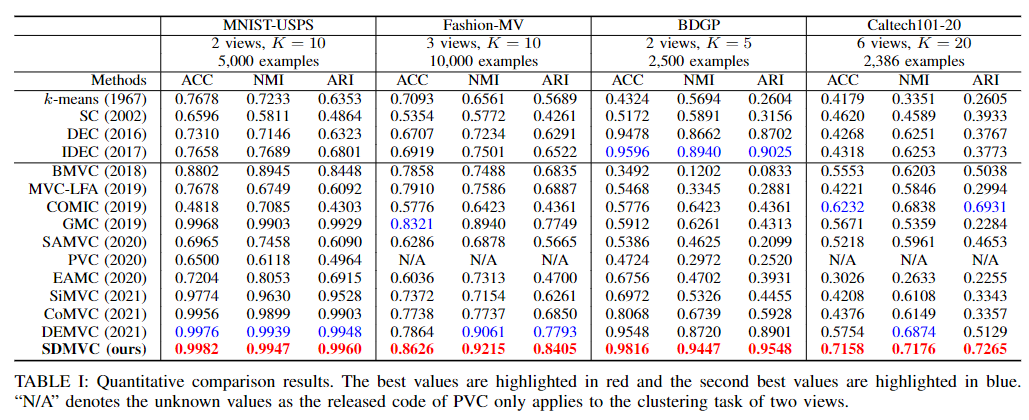
\includegraphics[width=\linewidth]{./imgs/img3.png}
\end{figure}

\subsubsection*{C. 实现细节}
我们分别应用全连接(Fc)和卷积(Conv)神经网络进行SDMVC的测试。

对于BDGP和Caltech101-20, 由于它们的所有视图都是矢量数据, 我们使用与[19]、[21]相同的全连接自编码器(FAE)。对于每个视图, 编码器为:输入 − Fc500 − Fc500 − Fc2000 − Fc10。对于MNIST-USPS和Fashion-MV, 我们遵循[14]、[25], 并为每个视图使用相同类型的卷积自编码器(CAE)来学习嵌入特征。编码器为:输入 − Conv5-32 − Conv5-64 − Conv3-128 − Fc10。这表示卷积核大小为5-5-3, 通道数为32-64-128。步幅为2。解码器与相应视图的编码器对称。以下设置对所有实验数据集相同。所有视图的嵌入特征维度被减少到10。ReLU [49] 作为激活函数, Adam [50](默认学习率为0.001)作为优化器。多视图自编码器预训练500个epoch。权衡系数 $\gamma$ 设为0.1。批量大小为256。每微调1000批次后更新目标分布。停止条件是对齐率达到约90%。

SDMVC的实验在Windows PC上进行, 配置为GeForce RTX 2060 GPU(6GB缓存)和Intel (R) Core (TM) i5-9400F CPU @ 2.90GHz, 16.0GB RAM。

采用开源代码和相应的建议设置进行比较方法。它们的超参数如下。

具体来说, IDEC和DEMVC的权衡系数 $\gamma$ 为0.1。

对于BMVC, $r$ 为5, $\beta$ 为0.003, $\gamma$ 为0.01, $\lambda$ 为$10^{-5}$, 代码长度为128。对于MVC-LFA, 使用高斯核, $\lambda$ 为23。COMIC的邻居大小和$\epsilon(v)$ 分别为10和0.9。对于GMC, $k$ 和 $\lambda$ 分别经验设置为15和1。SAMVC的SPL控制参数$\lambda(v)$ 设置为每次迭代从每个视图中添加15%的样本。对于PVC, 对齐率设为100%, $\lambda$ 为100。EAMC、SiMVC和CoMVC的实现设置来自https://github.com/DanielTrosten/mvc。


\subsubsection*{D. 评估指标}

使用的定量指标包括无监督聚类准确性(ACC)、归一化互信息(NMI)和调整兰德指数(ARI)。报告的结果是10次运行的平均值。ACC/NMI/ARI的较大值表示更好的聚类性能。

\subsection{结果和分析}

\subsubsection*{A. 真实数据上的结果}

我们提出的框架适用于卷积和全连接自编码器。因此, 图像数据输入卷积自编码器, 矢量数据输入全连接自编码器。然而, 有些算法无法处理原始图像数据, 因此数据被重新形状为矢量输入。定量比较如表I所示。可以观察到:(1) 我们的SDMVC在所有数据集上的定量指标上都取得了最佳性能。同时, 我们发现当使用5%的显著性水平进行t检验时, 改进是显著的。特别是在Fashion-MV, BDGP和Caltech101-20上, SDMVC大幅度改进了现有方法。(2) 一般来说, 单视图方法(k-means, SC, DEC和IDEC)的聚类性能比多视图方法差。然而, 在BDGP和Caltech101-20上, 比较的MVC方法的性能也有限。特别是在BDGP上, 一些MVC方法的性能甚至低于单视图方法。原因是多个视图的维度变化很大, 即在BDGP上是1750/79, 在Caltech101-20上是48/40/254/1984/512/928。多个视图的判别性差异很大, 某些视图的聚类结构高度不清晰(我们将在V-B节中分析), 这在这些多视图聚类方法中造成了不可避免的负面影响。即便如此, SDMVC还是实现了最先进的聚类性能。其原因在于, 我们的方法中, 每个视图的训练是独立的, 目标分布是从全局视角生成的。首先, 可以克服低判别性视图带来的负面影响。然后, 减少了多个视图的干扰, 并保留了它们特征的多样性, 从而可以挖掘更多的补充信息来提高聚类性能。

\subsubsection*{B. 消融研究}

\begin{figure}[h]
    \centering
    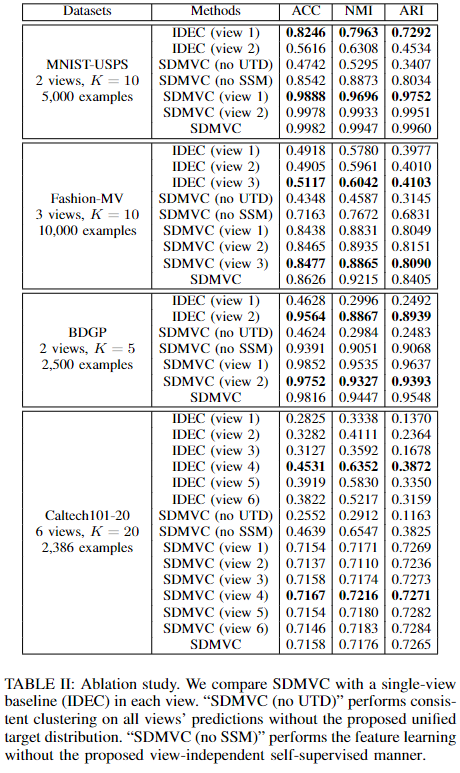
\includegraphics[width=0.4\linewidth]{./imgs/img5.png}
\end{figure}


我们测试了IDEC在每个独立视图上的聚类性能。表II所示, IDEC的最佳视图和最差视图之间的性能差距相当大, 低聚类性能表明它们的聚类结构不清晰。
在没有标签信息的情况下, 我们不确定哪个视图的预测更好。
IDEC的最佳视图和SDMVC的相应视图用粗体显示。

我们发现SDMVC在MNIST-USPS上提高了约15\%, 在Fashion-MV上提高了30\%, 在BDGP上提高了3\%, 在Caltech101-20上提高了30\%。最终, SDMVC在所有视图上的聚类性能(即使是聚类性能最差的视图)也远远优于IDEC。这表明:(1) 我们的方法克服了低判别性视图带来的负面影响, 这些视图的聚类结构不清晰。(2) 在我们的方法中, 多个视图为彼此提供了补充信息, 从而提高了聚类性能。

我们还测试了SDMVC的两个变体:(1) "SDMVC (no UTD)" 没有产生满意的结果, 它在没有使用提出的统一目标分布(UTD)的情况下进行多个视图预测的一致聚类。相反, SDMVC中使用统一目标分布来学习一致的预测。通过平均多个视图的预测, SDMVC获得了明确的预测, 其聚类性能与SDMVC的最佳视图相当甚至更好。(2) "SDMVC (no SSM)" 相对于IDEC的改进也有限, 它在没有使用提出的视图独立自监督方式(SSM)的情况下进行特征学习。然而, 在SDMVC中, 每个视图的判别特征和聚类质心的学习是独立于其他视图的, 连接的低维嵌入特征仅用于获得伪标签信息。该框架保留了多个视图的多样性, 同时挖掘它们的补充信息, 从而大大提高了所有视图的聚类性能。因此, SDMVC的两个变体验证了其不同部分具有必要的贡献。

\subsubsection*{C. 模型分析}

我们在BDGP数据集上进行了模型分析。在图4(a)中, 我们可以发现对齐率和聚类性能呈正相关。在图4(b)中, 每次更新目标分布时, 新生成并增强的伪软分配具有更强的判别力。因此, 聚类损失(即KL散度)值突然增加。然后, 由于统一目标分布, 所有视图的软聚类分配被训练为一致, 从而提高了多个视图预测的对齐率。在图3中, 我们通过t-SNE [41] 可视化了BDGP上的嵌入特征学习过程。每个视图的聚类质心也被绘制出来, 它们是聚类层中的可学习参数, 即$\{\mu^v_j\}_{j=1, v=1}^{K, V}$。当自编码器的预训练完成后, BDGP的两个视图的嵌入特征分别如图3(a)和(e)所示。特征的判别度低, 聚类质心无法反映真实的聚类结构, 对应于图4(a)中的低NMI值和低对齐率(当$\#Batches=0$时)。通过挖掘两个视图中包含的全局判别信息, SDMVC构建了一个目标分布, 以学习更多判别特征, 反过来用于更新目标分布。因此, 在接下来的特征学习过程中, 嵌入特征的聚类结构变得越来越清晰, 同时它们的质心逐渐分离, 对应于高NMI值和高对齐率。上述观察验证了SDMVC通过执行提出的多视图判别特征学习来提高聚类性能的机制, SDMVC能够全局利用判别和补充信息, 同时克服某些视图聚类结构不清晰对聚类造成的负面影响。

正如图4(b)所示, 算法在每次更新目标分布后具有良好的收敛性。由于SDMVC的对齐率是以无监督方式计算的, 我们建议通过选择一个较高的值, 如90%, 来停止训练, 以保证多视图聚类的一致性。权衡系数$\gamma$的设置遵循那些使用聚类和重构之间权衡策略的方法(例如, [19]和[14]), 即$\gamma=0.1$。因此, SDMVC没有需要仔细调整的超参数。


\begin{figure}[h]
    \centering
    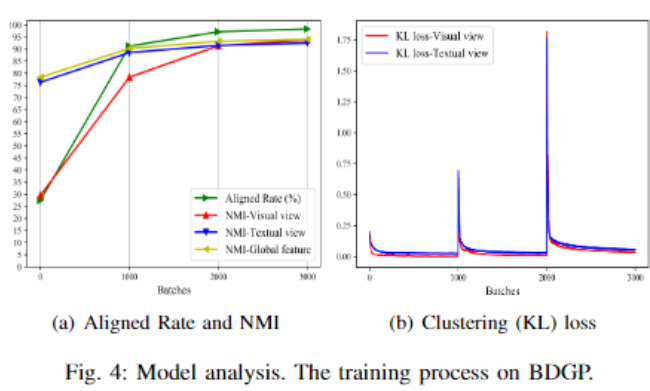
\includegraphics[width=0.75\linewidth]{./imgs/img4.png}
\end{figure}


\subsection{结论}
在本文中,我们提出了一种新颖的自监督判别特征学习框架用于深度多视图聚类 (SDMVC)。不同于现有的MVC方法,SDMVC能够克服某些视图聚类结构不清晰对聚类性能造成的负面影响。通过自监督方式,它利用全局视角的判别信息建立统一目标分布,用于学习更多判别特征和多个视图的一致预测。对不同类型多视图数据集的实验表明,所提出的方法实现了最先进的聚类性能。此外,SDMVC的复杂度与数据规模成线性关系,因此具有广泛的应用潜力。


\newpage

\section{总结思考}
本文介绍了一个基于自监督判别特征学习的深度多视图聚类方法(SDMVC),该方法充分利用了多个视图间的互补信息以提高聚类性能。与现有的多视图聚类方法相比,SDMVC在多个公认的数据集上展示了卓越的性能,证明了其在处理具有复杂分布的多视图数据中的有效性和鲁棒性。

成就:SDMVC方法通过在每个视图中独立训练并引入统一目标分布,有效地克服了视图之间的聚类结构不清晰的负面影响,同时保持了视图特征的多样性。此外,该方法的聚类性能不仅依赖于全局判别信息的有效利用,还体现在它能够通过自监督学习逐步优化特征表示,从而实现更一致的预测结果。

局限性:尽管SDMVC显示出了优异的聚类性能和较好的收敛性,但该方法的成功仍部分依赖于合理初始化和目标分布的准确更新。不适当的初始化或目标分布的更新可能会导致聚类性能下降。此外,虽然该方法在多个数据集上验证了其有效性,但对于那些极度不平衡或视图差异极大的数据集,SDMVC的表现和适应性仍需进一步研究。

未来研究方向:未来的工作可以在以下几个方面进行:首先,研究更先进的特征表示和自编码器结构,以提高模型在处理极端视图差异情况下的稳定性和准确性。其次,探索自动参数调整机制,以降低模型对初始配置的敏感性,使模型更加智能和用户友好。最后,将此框架扩展到半监督和有监督的多视图学习任务,可能会开辟新的研究和应用前景。

在完成这项研究后,我对多视图聚类的复杂性和挑战有了更深入的理解。尽管SDMVC在多个方面取得了显著的成效,但在实践中,每一步的实施都需要精心考量,确保每个视图的独立特性得到充分利用,同时又不丢失它们之间的互补信息。

通过这个项目,我更加意识到,在多视图环境中,不同视图可能呈现出相异的数据特征和分布。例如,一些视图可能包含更多的噪声,或者它们的聚类结构不如其他视图明显。SDMVC通过建立一个统一的目标分布来克服这些差异,这是一个非常聪明的设计。然而,这也引出了一个问题:我们如何确保这个统一目标分布始终有效并且反映了所有视图中的共同信息呢?这一点尤其在数据更新频繁或视图之间差异极大的实际应用中显得尤为重要。

此外,尽管算法的性能在当前的测试集上表现良好,但这是否意味着它将普遍适用于所有类型的多视图数据集仍有待观察。每个数据集都有其独特性,这可能会影响算法的聚类效果。因此,未来的研究需要更多地关注算法的泛化能力,探索在不同类型和规模的数据集上应用SDMVC的效果。

进一步思考,虽然我们目前侧重于无监督学习框架,将来我们可以考虑如何将有监督的学习元素融入框架中,以利用少量的标签数据来指导聚类过程。这种半监督学习方法可能会进一步提高模型的精确度和鲁棒性,特别是在复杂或边缘化的聚类情况下。

最后,我深刻认识到,技术和理论的进步需要与实际问题的需求紧密结合。我们的研究不应只关注算法本身,更应该考虑如何将这些算法应用到真实世界的问题中,解决具体的业务或社会挑战。通过这种方式,我们的工作才能真正达到科学研究的最终目的——服务于社会。


\section{原文}
\includepdf[pages=-]{./original_paper.pdf}
\end{document}



